\begin{quote}
Although a grounding in learning theory helps inform peer learning
projects, Peeragogy, at its core, comes to life in applied practice.
Even before convening a group for your peer learning project (discussed
in \href{http://peeragogy.github.io/convening.html}{Part IV}), you will
want to take a look over the patterns we have collected. You will likely
return here many times as your project develops.
\end{quote}

\hypertarget{what-is-a-pattern}{%
\subsection{What is a pattern?}\label{what-is-a-pattern}}

A pattern is anything that has a repeated effect. In the context of
peeragogy, the practice is to repeat processes and interactions that
advance the learning mission. Frequent occurrences that are not
desirable are called anti-patterns!

\begin{quote}
\textbf{Christopher Alexander}: ``Each pattern describes a problem which
occurs over and over again in our environment, and then describes the
core of the solution to that problem, in a way that you can use this
solution a million times over, without ever doing it the same way
twice.'' {{[}1{]}}
\end{quote}

Patterns provide a framework that can be applied to similar issues but
may be metaphorically solved in different ways, sometimes in real world
or face to face events and other times in digital space.~ Outside of
Alexander's own work in architecture, one the first groups to adopt a
design pattern way of thinking about things were computer programmers.~
Writing in the foreward to Richard P. Gabriel's \emph{Patterns of
Software}, Alexander emphasizes that the key question to ask about any
design approach is: does it help us build better?

\begin{quote}
\textbf{Christopher Alexander}: ``What is the Chartres of programming?
What task is at a high enough level to inspire people writing programs,
to reach for the stars?'' {{[}2{]}}
\end{quote}

We think that Peeragogy stands a good chance of being a~``killer app''
for pattern-based design.~ Learning bridges physical and virtual worlds
all the time.~ And, in fact, a \emph{Network of Learning} was the 18th
pattern that Christopher Alexander introduced in his book, \emph{A
Pattern Language}.

\begin{quote}
\textbf{Christopher Alexander}: ``Work in piecemeal ways to decentralize
the process of learning and enrich it through contact with many places
and people all over the city: workshops, teachers at home or walking
through the city, professionals willing to take on the young as helpers,
older children teaching younger children, museums, youth groups
travelling, scholarly seminars, industrial workshops, old people, and so
on.'' {{[}1{]}}
\end{quote}

Peeragogy can help to extend and enrich this network, and, as we shall
see, patterns can be used by those involved to do ongoing ``emergent''
design, not only by building new structures, but by adapting and
improving our catalog of patterns as we go.~ For consistency, and easy
use, adaptation, and extension we present the patterns using the
following template.~ The format is meant to be neutral and easy to work
with -- it's, intentionally, an outline that you might use to write a
short abstract describing an active project.

\begin{quote}
\textbf{Title}: \emph{Encapsulate the idea - possibly include a
subtitle}

\textbf{Context}: \emph{Describe the context in which it is meaningful.
What are the key \textbf{forces} acting in this context?}

\textbf{Problem}: \emph{Explain why there's some issue to address here.}

\textbf{Solution}: \emph{Talk about an idea about how to address the
issue.}

\textbf{Rationale}: \emph{Why do we use this solution as opposed to some
other solution?}

\textbf{Resolution}: \emph{How are the key forces resolved when the
solution is applied?}

\textbf{What's Next}: \emph{Talk about specific next steps. How will the
active forces continue to resolve in our project?}

Patterns include the following optional elements:

{{[}\textbf{Examples}: \emph{Present example(s) that have been
encountered, if this aids comprehension.}{]}}

{{[}\textbf{References}: \emph{Citations, if relevant.}{]}}
\end{quote}

The ``What's Next'' section concretely links the patterns we discuss
here to the Peeragogy project. It can be thought of as an annotation
rather than part of the pattern itself. If you adapt the patterns for
use in your own project, you're likely to have a different set of next
steps. Although we think that these patterns can be generally useful,
they aren't useful in the abstract, but rather, as a way for discussing
what we actually do.

\hypertarget{a-peeragogy-pattern-language}{%
\subsection{A peeragogy pattern
language}\label{a-peeragogy-pattern-language}}

By looking at how patterns combine in real and hypothetical use cases,
you can start to identify a \emph{pattern language} that can be used in
your projects. We can get a simplified view of these connections with
the following diagram.~ It's important to clarify that everyone doesn't
do it the same way.~ Here, the \emph{Roadmap} is given a central
position, but some peer learning projects will forego making a specific,
detailed plan; their plan is just to see what develops. You can see here
how peeragogy patterns often break down further into individual
micro-steps: we'll say more about that shortly.

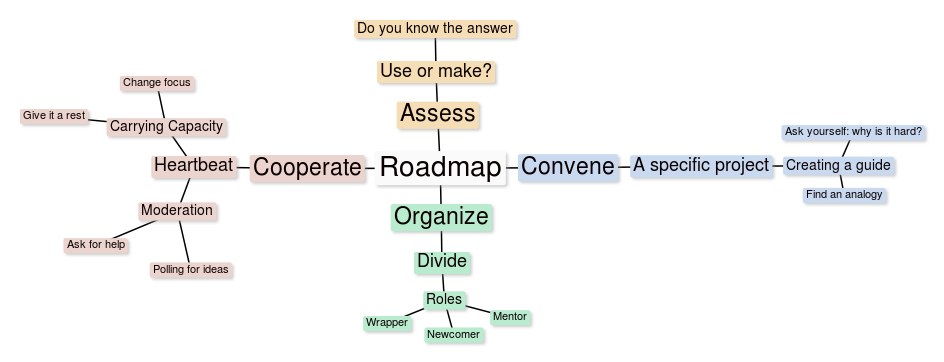
\includegraphics{images/pattern-language.jpg} {[}can this chart be
larger? Looks very small in text{]} The subsequent main sections of this
book -- \href{http://peeragogy.org/convene/}{\emph{Convene}},
\href{http://peeragogy.org/organize/}{\emph{Organize}},
\href{http://peeragogy.org/facilitate/}{\emph{Cooperate}} and
\href{http://peeragogy.org/assessment/}{\emph{Assess}} (for short) --
represent big clusters of patterns that are likely to come up time and
again in various projects.~ We can think of these as East, South, West,
and North in the diagram above. You are encouraged to invent your own
patterns and to connect them in new ways. You'll probably find quite a
few that we didn't include in the catalog. Each project has a unique
design, and it's own unique way in which things play out in practice.
What we've put together here is a starter kit. The peeragogy patterns
suggest a social way to do problem solving {[}3{]}, but once you get
used to the pattern concept you can use it to identify new problems no
one has ever thought of before, and that's even more powerful!

\hypertarget{references}{%
\subsection{References}\label{references}}

\begin{enumerate}
\def\labelenumi{\arabic{enumi}.}
\item
  Alexander, C., Ishikawa, S., and Silverstein, M. (1977). \emph{A
  Pattern Language: Towns, Buildings, and, Construction}, New York:
  Oxford University Press.
\item
  Gabriel, Richard P. (1996).
  \emph{\href{http://dreamsongs.net/Files/PatternsOfSoftware.pdf}{Patterns
  of Software}}, New York: Oxford University Press. (Includes a foreward
  by Christopher Alexander.)
\item
  Minsky, Marvin. (2008--2009). \emph{Essays on Education (for
  {O}{L}{P}{C})}, Massachusetts Institute of Technology Media Lab
  whitepaper,
  \href{http://web.media.mit.edu/~minsky/OLPC-1.html}{Available online.}
\end{enumerate}
